\documentclass{article}
\usepackage{amsmath}
\usepackage{amsthm}
\usepackage{amssymb}
\usepackage{algorithm}
\usepackage{algorithmic}
\usepackage{dirtytalk}
\usepackage{enumerate}
\usepackage[margin=1.00in]{geometry}
\usepackage{graphicx}
\usepackage{hyperref}
\usepackage{optidef}
\usepackage{tikz}

% define colors
\definecolor{white}{RGB}{255,255,255} % white
\definecolor{gray}{RGB}{192,192,192} % gray
\definecolor{black}{RGB}{0,0,0} % black
\definecolor{sky_blue}{RGB}{135,206,250} % sky blue

% new theorems and definitions
\newtheorem{theorem}{Theorem}[section]
\newtheorem{proposition}[theorem]{Proposition}
\newtheorem{corollary}[theorem]{Corollary}
\newtheorem{lemma}[theorem]{Lemma}
\newtheorem{question}[theorem]{Question}
\theoremstyle{definition}
\newtheorem{remark}[theorem]{Remark}

% new commands and math operators
\newcommand\abs[1]{\left|#1\right|}
\newcommand*\conj[1]{\overline{#1}}
\newcommand\nullity[1]{\operatorname{nullity}\left(#1\right)}
\newcommand\kernel[1]{\operatorname{null}\left(#1\right)}
\newcommand\rank[1]{\operatorname{rank}\left(#1\right)}
\newcommand\zip[1]{\operatorname{ZIP}\left(#1\right)}

\title{On Zero Forcing and the Inverse Eigenvalue Problem for Graphs}
\author{Thomas R. Cameron}
\date{\today}

\begin{document}
\maketitle
\abstract{This note is intended to introduce the connection between the inverse eigenvalue problem of a graph and the zero forcing number of a graph.}
%%%%%%%%%%%%%%%%%%%%%%%%%%%%%%%%%%%%%%%%%%%%%%%%%%%%%%
%                                    				Introduction
%%%%%%%%%%%%%%%%%%%%%%%%%%%%%%%%%%%%%%%%%%%%%%%%%%%%%%
\section{Introduction}	\label{sec:intro}
Let $\mathbb{G}$ denote the collection of all simple graphs (no loops nor multi-edges) of order $n$.
With each graph $G\in\mathbb{G}$, there is a vertex set $V(G) = \{v_{1},v_{2},\ldots,v_{n}\}$ and an edge set $E(G)$, where $\{v_{i},v_{j}\}\in E(G)$ if and only if $i\neq j$ and $v_{i}$ and $v_{j}$ are adjacent vertices.
For example, let $G$ be the star graph of order $7$ shown in Figure~\ref{fig:star-graph}.
Then, $V(G) = \{1,2,3,4,5,6,7\}$ and $E(G) = \{\{1,7\},\{2,7\},\{3,7\},\{4,7\},\{5,7\},\{6,7\}\}$. 

%%%%%%%%%%%%%%%%
%					Figure 1				%
%%%%%%%%%%%%%%%%
\begin{figure}[ht]
\centering
\resizebox{0.20\textwidth}{!}{% Star Graph
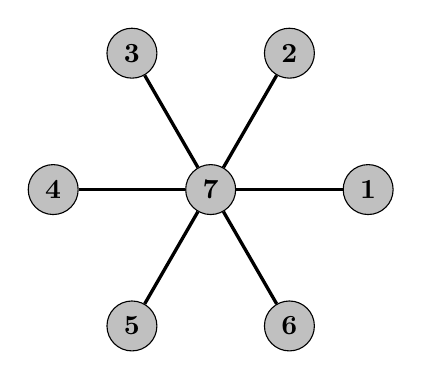
\begin{tikzpicture}
	\node[circle,draw=black,fill=gray] (1) at (2,0) {\textbf{1}};
	\node[circle,draw=black,fill=gray] (2) at (1,1.732) {\textbf{2}};
	\node[circle,draw=black,fill=gray] (3) at (-1,1.732) {\textbf{3}};
	\node[circle,draw=black,fill=gray] (4) at (-2,0) {\textbf{4}};
	\node[circle,draw=black,fill=gray] (5) at (-1,-1.732) {\textbf{5}};
	\node[circle,draw=black,fill=gray] (6) at (1,-1.732) {\textbf{6}};
	\node[circle,draw=black,fill=gray] (7) at (0,0) {\textbf{7}};
	
	\foreach \x/\y in {7/1,7/2,7/3,7/4,7/5,7/6}
		\draw[black,=>latex',very thick] (\x) -- (\y);
\end{tikzpicture}%
}
\caption{A star graph of order $7$.}
\label{fig:star-graph}
\end{figure}

Every $n\times n$ symmetric matrix $A=[a_{ij}]_{i,j=1}^{n}$ is associated with a graph $G\in\mathbb{G}$, where $a_{ij}\neq 0$ if and only if $\{v_{i},v_{j}\}\in E(G)$.
Given a graph $G\in\mathbb{G}$, the set of all $n\times n$ symmetric matrices associated with $G$ is denoted by
\[
\mathcal{S}(G) = \left\{A=[a_{ij}]_{i,j=1}^{n}\colon a_{ij}=a_{ji}~\forall i\neq j,~a_{ij}\neq 0~\Leftrightarrow~\{v_{i},v_{j}\}\in E(G)\right\}.
\]
For example, the star graph $G$ shown in Figure~\ref{fig:star-graph} is associated with symmetric matrices of the form
\[
A = \begin{bmatrix} 
		\alpha_{1} & 0 & \cdots & 0 & \beta_{1} \\
		0 & \alpha_{2} & \cdots & 0 & \beta_{2} \\
		\vdots & & \ddots & &  \vdots \\
		0 & & & \alpha_{6} & \beta_{6} \\
		\beta_{1} & \beta_{2} & \cdots & \beta_{6} & \alpha_{7} \\
	\end{bmatrix}.
\]

The inverse eigenvalue problem of a graph can be stated as follows:
Given a graph $G\in\mathbb{G}$, what are all possible length $n$ multi-sets $\sigma$ such that there is a matrix $A\in\mathcal{S}(G)$ with spectrum $\sigma$.
This important question is obviously difficult to answer in general; however, there are a few observations we can make. 
\begin{itemize}
\item  The empty graph of order $n$, denoted $E_{n}$, has no edges.
		Therefore, $\mathcal{S}(E_{n})$ is the set of all $n\times n$ diagonal matrices.
		Since the eigenvalues of a diagonal matrix are equal to its diagonal entries, it follows that every length $n$ multi-set $\sigma$ corresponds to the eigenvalues of a matrix $A\in\mathcal{S}(E_{n})$.
		It turns out, that the empty graph is the only graph with this property. 
\item Let $K_{n}$ denote a complete graph of order $n$.
		Then, $\mathcal{S}(K_{n})$ is made up of symmetric matrices where all off-diagonal entries are non-zero. 
		Furthermore, for any $\lambda_{1}\leq\lambda_{2}\leq\cdots\lambda_{n}$, there is a matrix $A\in\mathcal{S}(K_{n})$ with eigenvalues $\lambda_{1},\lambda_{2},\ldots,\lambda_{n}$ if and only if $\lambda_{1}<\lambda_{n}$~\cite{Barrett2013}.
\item Let $P_{n}$ denote a path graph of order $n$.
		Then, $\mathcal{S}(P_{n})$ corresponds to tri-diagonal matrices with non-zero entries in the upper and lower diagonals.
		Furthermore, any length $n$ multi-set $\sigma$ corresponds to the eigenvalues of a matrix $A\in\mathcal{S}(P_{n})$ if and only if the entries of $\sigma$ are distinct~\cite{Hochstadt1967}.
\end{itemize}

Due to the difficulty of the inverse eigenvalue problem of a graph, there is a focus on solving related but seemingly easier problems.
For instance, one may want to find the maximum multiplicity of a graph $G\in\mathbb{G}$, denoted $M(G)$, which is defined as the largest integer $k$ such that there is a matrix $A\in\mathcal{S}(G)$ with an eigenvalue of multiplicity $k$.
Note $M(E_{n})=n$, $M(K_{n})=(n-1)$,  and $M(P_{n})=1$.

The multiplicity of an eigenvalue $\lambda$ of the symmetric matrix $A$ is equal to the nullity of $\lambda I - A$, i.e,  the dimension of the null space of $\lambda I-A$.
Note that for any $A\in\mathcal{S}(G)$, it follows that $\lambda I - A\in\mathcal{S}(G)$.
Therefore,
\[
M(G) = \max\left\{\nullity{A}\colon A\in\mathcal{S}(G)\right\}.
\]
For this reason, the maximum multiplicity of a graph is often refereed to as the max nullity of the graph. 

In a similar manner, the minimum rank of $G$, denoted $mr(G)$, is defined by 
\[
mr(G) = \min\left\{\rank{A}\colon A\in\mathcal{S}(G)\right\}.
\]
Recall that the $\rank{A}$ is the dimension of the column space of $A$.
By the rank-nullity theorem, we have
\[
mr(G) + M(G) = n.
\]

In 2006, at the AIMS Workshop on \say{Spectra of families of matrices described by graphs, digraphs, and sign pattern}, a novel connection between the maximum nullity of a graph and its zero forcing number was presented. 
Zero forcing was introduced independently by Burgarth and Giovannetti in the control of quantum systems~\cite{Burgarth2007}, where it was called graph infection.
For our purposes, zero forcing is a coloring game on a graph, where an initial set of vertices are colored blue and all other vertices are colored white.
Then, the blue vertices force neighboring white vertices blue using a color change rule.
There are many color changing rules, but the standard rule is that a blue vertex $b$ can force a white vertex $w$ blue if $w$ is the only white neighbor of $b$.
We will reference this rule as the Z-color change rule to distinguish it from the other variants. 

%%%%%%%%%%%%%%%%%%%%%%%%%%%%%%%%%%%%%%%%%%%%%%%%%%%%%%
%                                    				Zero-Forcing
%%%%%%%%%%%%%%%%%%%%%%%%%%%%%%%%%%%%%%%%%%%%%%%%%%%%%%
\section{Zero-Forcing}\label{sec:zf}
Given a  graph $G\in\mathbb{G}$, let $B\subseteq V(G)$ denote the initial set of blue vertices; this is called the initial coloring of $G$.
Then, denote by $B^{[t]}$ the blue vertices after $t$ applications of the Z-color change rule, where $B^{[0]}=B$.
Because the graph is finite, there exists a $t^{*}\geq 0$ for which $B^{[t^{*}]} = B^{[t^{*}+k]}$, for all $k\in\mathbb{N}$, i.e., no more changes are possible from applying the Z-color change rule. 
We reference $B^{[t^{*}]}$ as the final coloring of $B$.
If $B^{[t^{*}]} = V(G)$, i.e., the final coloring is all of the vertices of $G$, then we say that $B$ is a zero forcing set of $G$.
The zero forcing number of $G$ is defined as the cardinality of the smallest zero forcing set of $G$:
\[
Z(G) = \min\left\{\abs{B}\colon B^{[t^{*}]} = V(G)\right\}.
\]

For example, consider the application of the Z-color change rule to a path graph on $5$ vertices shown in Figure~\ref{fig:path-graph-coloring}.
It is clear that $B^{[4]}$ is the final coloring of $B$ since $B^{[5]} = B^{[4]}$.
Furthermore, since $B^{[4]}$ encompasses all vertices in the graph, it follows that $B=\{1\}$ is a zero forcing set and, hence, the zero forcing number of this path graph is equal to $1$.
%%%%%%%%%%%%%%%%
%					Figure 2			%
%%%%%%%%%%%%%%%%
\begin{figure}[ht]
\centering
\resizebox{0.75\textwidth}{!}{% Path Graph Coloring
\begin{tabular}{ccc}
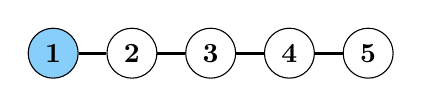
\begin{tikzpicture}
	\node[circle,draw=black,fill=sky_blue] (1) at (-2,0) {\textbf{1}};
	\node[circle,draw=black,fill=white] (2) at (-1,0) {\textbf{2}};
	\node[circle,draw=black,fill=white] (3) at (0,0) {\textbf{3}};
	\node[circle,draw=black,fill=white] (4) at (1,0) {\textbf{4}};
	\node[circle,draw=black,fill=white] (5) at (2,0) {\textbf{5}};
	
	\foreach \x/\y in {1/2,2/3,3/4,4/5}
		\draw[black,=>latex',very thick] (\x) -- (\y);
\end{tikzpicture}
&
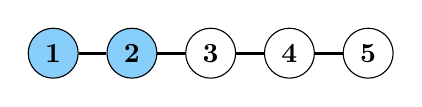
\begin{tikzpicture}
	\node[circle,draw=black,fill=sky_blue] (1) at (-2,0) {\textbf{1}};
	\node[circle,draw=black,fill=sky_blue] (2) at (-1,0) {\textbf{2}};
	\node[circle,draw=black,fill=white] (3) at (0,0) {\textbf{3}};
	\node[circle,draw=black,fill=white] (4) at (1,0) {\textbf{4}};
	\node[circle,draw=black,fill=white] (5) at (2,0) {\textbf{5}};
	
	\foreach \x/\y in {1/2,2/3,3/4,4/5}
		\draw[black,=>latex',very thick] (\x) -- (\y);
\end{tikzpicture}
&
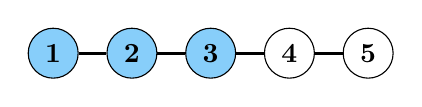
\begin{tikzpicture}
	\node[circle,draw=black,fill=sky_blue] (1) at (-2,0) {\textbf{1}};
	\node[circle,draw=black,fill=sky_blue] (2) at (-1,0) {\textbf{2}};
	\node[circle,draw=black,fill=sky_blue] (3) at (0,0) {\textbf{3}};
	\node[circle,draw=black,fill=white] (4) at (1,0) {\textbf{4}};
	\node[circle,draw=black,fill=white] (5) at (2,0) {\textbf{5}};
	
	\foreach \x/\y in {1/2,2/3,3/4,4/5}
		\draw[black,=>latex',very thick] (\x) -- (\y);
\end{tikzpicture}
\\ $B^{[0]} = \{1\}$ & $B^{[1]} = \{1,2\}$ & $B^{[2]} = \{1,2,3\}$ \\
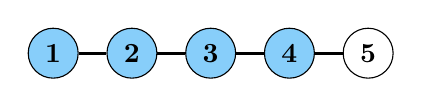
\begin{tikzpicture}
	\node[circle,draw=black,fill=sky_blue] (1) at (-2,0) {\textbf{1}};
	\node[circle,draw=black,fill=sky_blue] (2) at (-1,0) {\textbf{2}};
	\node[circle,draw=black,fill=sky_blue] (3) at (0,0) {\textbf{3}};
	\node[circle,draw=black,fill=sky_blue] (4) at (1,0) {\textbf{4}};
	\node[circle,draw=black,fill=white] (5) at (2,0) {\textbf{5}};
	
	\foreach \x/\y in {1/2,2/3,3/4,4/5}
		\draw[black,=>latex',very thick] (\x) -- (\y);
\end{tikzpicture}
&
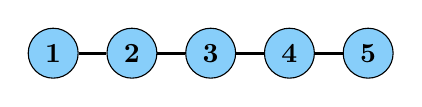
\begin{tikzpicture}
	\node[circle,draw=black,fill=sky_blue] (1) at (-2,0) {\textbf{1}};
	\node[circle,draw=black,fill=sky_blue] (2) at (-1,0) {\textbf{2}};
	\node[circle,draw=black,fill=sky_blue] (3) at (0,0) {\textbf{3}};
	\node[circle,draw=black,fill=sky_blue] (4) at (1,0) {\textbf{4}};
	\node[circle,draw=black,fill=sky_blue] (5) at (2,0) {\textbf{5}};
	
	\foreach \x/\y in {1/2,2/3,3/4,4/5}
		\draw[black,=>latex',very thick] (\x) -- (\y);
\end{tikzpicture}
&
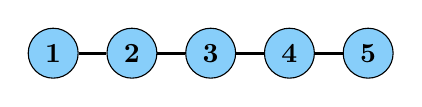
\begin{tikzpicture}
	\node[circle,draw=black,fill=sky_blue] (1) at (-2,0) {\textbf{1}};
	\node[circle,draw=black,fill=sky_blue] (2) at (-1,0) {\textbf{2}};
	\node[circle,draw=black,fill=sky_blue] (3) at (0,0) {\textbf{3}};
	\node[circle,draw=black,fill=sky_blue] (4) at (1,0) {\textbf{4}};
	\node[circle,draw=black,fill=sky_blue] (5) at (2,0) {\textbf{5}};
	
	\foreach \x/\y in {1/2,2/3,3/4,4/5}
		\draw[black,=>latex',very thick] (\x) -- (\y);
\end{tikzpicture}
\\ $B^{[3]} = \{1,2,3,4\}$ & $B^{[4]} = \{1,2,3,4,5\}$ & $B^{[5]} = \{1,2,3,4,5\}$ \\
\end{tabular}%
}
\caption{A zero forcing set for a path graph of order $5$.}
\label{fig:path-graph-coloring}
\end{figure}

One can easily generalize the above example and conclude that the zero forcing number of all path graphs is equal to $1$, i.e., $Z(P_{n}) = 1$.
Note that not every initial coloring of $1$ vertex is a zero forcing set of $P_{n}$. 
Indeed, consider the initial coloring of a path graph on $5$ vertices shown in Figure~\ref{fig:path-graph-coloring2}.

%%%%%%%%%%%%%%%%
%					Figure 3			%
%%%%%%%%%%%%%%%%
\begin{figure}[ht]
\centering
\resizebox{0.25\textwidth}{!}{% Path Graph Coloring 2
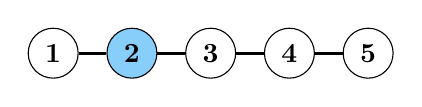
\begin{tikzpicture}
	\node[circle,draw=black,fill=white] (1) at (-2,0) {\textbf{1}};
	\node[circle,draw=black,fill=sky_blue] (2) at (-1,0) {\textbf{2}};
	\node[circle,draw=black,fill=white] (3) at (0,0) {\textbf{3}};
	\node[circle,draw=black,fill=white] (4) at (1,0) {\textbf{4}};
	\node[circle,draw=black,fill=white] (5) at (2,0) {\textbf{5}};
	
	\foreach \x/\y in {1/2,2/3,3/4,4/5}
		\draw[black,=>latex',very thick] (\x) -- (\y);
\end{tikzpicture}%
}
\caption{A non zero forcing set for a path graph of order $5$.}
\label{fig:path-graph-coloring2}
\end{figure}

We are now ready to present the connection between the zero forcing number and the maximum nullity of a graph.
First we require the following lemma. 
%%%%%%%%%%%%%%%%
%					Lemma 1.1			%
%%%%%%%%%%%%%%%%
\begin{lemma}\label{lem:non-zero-int}
Suppose that $\alpha\subseteq\{1,2,\ldots,n\}$ with $\abs{\alpha}<k$ and $U$ is a subspace of $\mathbb{R}^{n}$ of dimension $k$.
Then, $U$ contains a non-zero vector of $\textbf{v}$ with $\textbf{v}[\alpha] = 0$.
\end{lemma}
\begin{proof}
Note that if $U$ and $V$ are subspaces of $\mathbb{R}^{n}$ whose dimensions satisfy
\[
\dim{V} > n - \dim{U},
\]
then $U$ and $V$ must have a non-trivial intersection, i.e., there is a non-zero vector in $U\cap V$.
Now, define
\[
V = \left\{\textbf{v}\in\mathbb{R}^{n}\colon \textbf{v}[\alpha] = 0\right\},
\]
and note that $\dim{V} = n - \abs{\alpha} > n - k = \dim{U}$.
Hence, there exists a non-zero vector $\textbf{v}\in U\cap V$, and the result follows.
\end{proof}

%%%%%%%%%%%%%%%%
%					Theorem 1.2		%
%%%%%%%%%%%%%%%%
\begin{theorem}\label{thm:max-nul-zero-forcing}
Let $G\in\mathbb{G}$.
Then, $M(G)\leq Z(G)$.
\end{theorem}
\begin{proof}
Let $B\subseteq V(G)$ be a zero forcing set of $G$, and let $A\in\mathcal{S}(G)$.
If $\abs{B}<\nullity{A}$, then Lemma~\ref{lem:non-zero-int} implies that there exists a non-zero vector $\textbf{x}\in\kernel{A}$ such that $\textbf{x}_{i}=0$ for all $i\in B$.
However, if a vector $\textbf{x}\in\kernel{A}$ satisfies $\textbf{x}_{i}=0$ for all $i\in B$, then it follows that $\textbf{x}=\textbf{0}$.

Indeed, let $j\in V(G)\setminus{B}$ be any vertex that is forced by some $i\in B$; at least one such vertex must exist since $B$ is a zero forcing set.
Then, the equation $A\textbf{x}=\textbf{0}$ implies that $a_{ij}\textbf{x}_{j}=0$, which gives $\textbf{x}_{j}=0$ since $a_{ij}\neq 0$.
If necessary, we can repeat the above argument on the zero forcing set $B\cup\{j\}$, and perhaps again, until all vertices in $V(G)$ are accounted for at which point it follows that $\textbf{x}=\textbf{0}$.

This contradiction with Lemma~\ref{lem:non-zero-int} implies that $\abs{B}\geq\nullity{A}$.
Since $B$ and $A$ are arbitrary, it follows that $Z(G)\geq M(G)$.
\end{proof}

Theorem~\ref{thm:max-nul-zero-forcing} can be used to determine the maximum nullity of a graph via its zero forcing number. 
For instance, we know that the path graph satisfies $Z(P_{n})=1$.
Therefore, Theorem~\ref{thm:max-nul-zero-forcing} implies that $M(P_{n}) \leq 1$.
Since there is always a singular matrix in $\mathcal{S}(G)$, for any graph $G$, it follows that $M(P_{n})=1$.

As a more interesting example, consider the star graph in Figure~\ref{fig:star-graph}.
Note that $B=\{1,2,3,4,5\}$ is a zero-forcing set of minimal size. 
This observation can easily be generalized and we conclude that the zero forcing number of the star graph $K_{1,n-1}$ of order $n$ satisfies $Z(K_{1,n-1}) = n-2$.
Therefore, the maximum nullity and minimum rank satisfy
\[
M(K_{1,n-1}) \leq n-2~\text{and}~mr(K_{1,n-1}) \geq 2,
\]
respectively.
Furthermore, the adjacency matrix of the star graph $K_{1,n-1}$:
\[
A = \begin{bmatrix} 
		0 & 0 & \cdots & 0 & 1 \\
		0 & 0 & \cdots & 0 & 1 \\
		\vdots & & \ddots & &  \vdots \\
		0 & & & 0 & 1 \\
		1 & 1 & \cdots & 1 & 0 \\
	\end{bmatrix}.
\]
is a $n\times n$ matrix in $\mathcal{S}(K_{1,n-1})$ that satisfies $\rank{A} = 2$.
Therefore, $M(K_{1,n-1})=n-2$ and $mr(K_{1,n-2}) = 2$.

%%%%%%%%%%%%%%%%%%%%%%%%%%%%%%%%%%%%%%%%%%%%%%%%%%%%%%
%                                    				Known Values and Bounds
%%%%%%%%%%%%%%%%%%%%%%%%%%%%%%%%%%%%%%%%%%%%%%%%%%%%%%
\subsection{Known Values and Bounds}\label{subsec:zf-values-bounds}
It is worth pointing out that there are some classes of graphs for which the zero-forcing number is well known. 
In many of these cases, the bound in Theorem~\ref{thm:max-nul-zero-forcing} is sharp, see the list below. 
\begin{enumerate}[i.]
\item For any tree $T$, 
\[
Z(T) = M(T) = P(T),
\]
where $P(T)$ denotes the path cover number, i.e., the minimum number of paths in a path cover of $T$.
\item For $n\geq 2$,
\[
Z(K_{n}) = M(K_{n}) = n-1. 
\]
\item For $n\geq 1$,
\[
Z(E_{n}) = M(E_{n}) = n.
\]
\item For $n\geq 3$,
\[
Z(C_{n}) = M(C_{n}) = 2,
\]
where $C_{n}$ is a cycle graph of order $n$. 
\item For $n\geq 3$,
\[
Z(\conj{C}_{n}) = M(\conj{C}_{n}) = n-3,
\]
where $\conj{\cdot}$ denotes the graph conjugate. 
\item For $n\geq 4$,
\[
Z(W_{n}) = M(W_{n}) = 3,
\]
where $W_{n}$ is a wheel graph of order $n$. Note that wheel graphs are formed by connecting a single vertex to all vertices in a cycle. 
\item For $p,q\geq 1$ and $p+q\geq 3$, 
\[
Z(K_{p,q}) = M(K_{p,q}) = p+q-2,
\]
where $K_{p,q}$ is a bipartite graph, i.e., the join of two empty graphs of order $p$ and $q$, respectively.
\item The Cartesian product of two graphs $G=(V,E)$ and $G'=(V',E')$, denoted $G\square G'$, is a graph on $V\times V'$ such that $(v,v')$ and $(u,u')$ are adjacent if and only if $v=u$ and $\{v',u'\}\in E'$, or $v'=u'$ and $\{v,u\}\in E$.  Note that we have the following known values for Cartesian products:
	\begin{enumerate}[a.]
	\item $Z\left(K_{n}\square P_{m}\right) = M\left(K_{n}\square P_{m}\right) = n$,
	\item $Z\left(P_{n}\square P_{m}\right) = M\left(P_{n}\square P_{m}\right) = \min\{n,m\}$,
	\item $Z\left(C_{n}\square P_{m}\right) = M\left(C_{n}\square P_{m}\right) = \min\{n,2m\}$,
	\item $Z\left(C_{n}\square K_{m}\right) = M\left(C_{n}\square K_{m}\right) = 2m$, for $n\geq 4$,
	\item $Z\left(K_{n}\square K_{m}\right) = M\left(K_{n}\square K_{m}\right) = m-n + 2$.
	\end{enumerate}
\end{enumerate}

We conclude with readily verifiable bounds on the zero-forcing number of a graph. 
Throughout, let $\delta(G)$ denote the minimum degree of a vertex in $G$ and let $\Delta(G)$ denote the maximum degree of a vertex in $G$.
%%%%%%%%%%%%%%%%
%					Proposition 2.3	%
%%%%%%%%%%%%%%%%
\begin{proposition}\label{prop:zf-bound}
If $G$ has at least one edge, then
\[
\delta(G) \leq Z(G) \leq n - 1.
\]
\end{proposition}

%%%%%%%%%%%%%%%%
%					Proposition 2.4	%
%%%%%%%%%%%%%%%%
\begin{proposition}\label{prop:zf-ubound}
If $\delta(G)\geq 1$, then 
\[
Z(G) \leq \frac{\Delta(G)}{\Delta(G)+1}n
\]
and if $\delta(G)\geq 2$, then
\[
Z(G) \leq \frac{\left(\Delta(G)-2\right)n+2}{\Delta(G)-1}.
\]
\end{proposition}

%%%%%%%%%%%%%%%%
%					Proposition 2.5	%
%%%%%%%%%%%%%%%%
\begin{proposition}\label{prop:zf-lbound}
If $G$ is a graph of order $n$, then
\[
Z(G) \geq \frac{\abs{E(G)}}{n}.
\]
\end{proposition}


%%%%%%%%%%%%%%%%%%%%%%%%%%%%%%%%%%%%%%%%%%%%%%%%%%%%%%
%                                    				Positive Semidefinite Zero Forcing
%%%%%%%%%%%%%%%%%%%%%%%%%%%%%%%%%%%%%%%%%%%%%%%%%%%%%%
\section{Positive Semidefinite Zero Forcing}\label{sec:psd-zf}
As mentioned in Section~\ref{sec:intro}, there are many color change rules that can be used in the coloring game of zero forcing. 
The so-called standard zero forcing rule provides an upper bound on the maximum nullity of a graph via Theorem~\ref{thm:max-nul-zero-forcing}.
The positive semidefinite zero forcing rule provides an upper bound on the maximum positive semidefinite nullity:
\[
M_{+}(G) = \max\left\{\nullity{A}\colon A\in\mathcal{S}(G),~\forall\lambda\in\sigma(A),~\lambda\geq 0\right\}.
\]
Note that the additional condition on the eigenvalues of $A$, i.e., $\lambda\geq 0$ for all $\lambda\in\sigma(A)$, implies that $A$ must be positive semidefinite. 
%Furthermore, because the eigenvalues must be non-negative, $M_{+}(G)$ no longer corresponds to the maximum multiplicity of an eigenvalue of a positive semidefinite matrix in $\mathcal{S}(G)$.

Given a graph $G\in\mathbb{G}$, let $B\subseteq V(G)$ denote the initial coloring of $G$. 
Let $G-B$ denote the resulting graph after the blue vertices (and adjacent edges) have been removed, and let $W_{1},\ldots,W_{k}$ denote the vertex sets of the connected components of $G-B$.
If $b\in B$ and $w\in W_{i}$ is the only white neighbor of $b$ in $G[W_{i}\cup B]$, for some $i\in\{1,\ldots,k\}$, then the positive semidefinite zero forcing rule says that $b$ can force $w$ blue.

As with the standard zero forcing rule, there exists a $t^{*}\geq 0$ such that $B^{[t^{*}]} = B^{[t^{*}+k]}$ for all $k\in\mathbb{N}$, and we say that $B$ is a positive semidefinite zero forcing set if the final coloring satisfies $B^{[t^{*}]} = V(G)$.
The positive semidefinite zero forcing number of $G$ is defined as the cardinality of the smallest positive semidefinite zero forcing set of $G$:
\[
Z_{+}(G) = \min\left\{\abs{B}\colon B^{[t^{*}]} = V(G)\right\}.
\]
%%%%%%%%%%%%%%%%
%					Theorem 2.1		%
%%%%%%%%%%%%%%%%
\begin{theorem}\label{thm:psd-max-nul-zero-forcing}
Let $G\in\mathbb{G}$.
Then, $M_{+}(G)\leq Z_{+}(G)$.
\end{theorem}
\begin{proof}
Let $A\in\mathcal{S}(G)$ be positive semidefinite with $\nullity{A}=M_{+}(G)$ and consider a non-zero vector $\textbf{x}\in\null{A}$, which is guaranteed to exist since the max nullity is at least $1$.
Let $B\subset V(G)$ denote the set of vertices such that $\textbf{x}_{i}=0$, and let $W_{1},\ldots,W_{k}$ denote the vertex sets of the connected components of $G\setminus{B}$.
For every $i\in\{1,\ldots,k\}$, we claim that no $w\in W_{i}$ can be the only neighbor of a $b\in B$ in $G[W_{i}\cup B]$.

Indeed, note that we can write $A$, possibly after re-ordering the vertices of $G$, as follows 
\[
A = \begin{bmatrix}
		A_{1} & 0 & \cdots & 0 & C_{1} \\
		0 & A_{2} & \cdots & 0 & C_{2} \\
		\vdots & \vdots & \ddots & \vdots & \vdots \\
		0 & 0 & \cdots & A_{k} & C_{k} \\
		C_{1} & C_{2} & \cdots & C_{k} & D \\
		\end{bmatrix},
\]
where $A_{1},\ldots,A_{k}$ corresponds to the vertex sets $W_{1},\ldots,W_{k}$, respectively, $D$ corresponds to the vertex set $B$, and $C_{i}$ corresponds to the edges between $W_{i}$ and $B$, for all $i\in\{1,\ldots,k\}$.

Now, consider the partition $\textbf{x} = [\textbf{x}_{1}^{T},\ldots,\textbf{x}_{k}^{T},\textbf{0}^{T}]$, where $\textbf{x}_{i}$ has size equal to $\abs{W_{i}}$, for all $i\in\{1,\ldots,k\}$, and the zero vector $\textbf{0}$ has size equal to $\abs{B}$.
Note that all entries of $\textbf{x}_{1},\ldots,\textbf{x}_{k}$ must be non-zero.
Moreover, the equation $A\textbf{x}=\textbf{0}$ implies that $A_{i}\textbf{x}_{i}=\textbf{0}$ for all $i\in\{1,\ldots,k\}$.

The column inclusion property for Hermitian positive semidefinite matrices~\cite{Johnson1998}, guarantees that each column in $C_{i}$ is the span of the columns in $A_{i}$, for all $i\in\{1,\ldots,k\}$.
Therefore, for each $i\in\{1,\ldots,k\}$, there exists a matrix $Y_{i}$ such that $C_{i}=A_{i}Y_{i}$.
Since $A$ is symmetric, it follows that $C_{i}=Y_{i}^{T}A_{i}$; hence, $C_{i}\textbf{x}_{i}=\textbf{0}$ for all $i\in\{1,\ldots,k\}$.
But if $w\in W_{i}$ were the only white neighbor of $b\in B$ in $G[W_{i}\cup B]$, then $C_{i}\textbf{x}_{i}\neq \textbf{0}$, which is a contradiction. 

This contradiction implies that $B$ is not a positive semidefinite zero forcing set of $G$.
Furthermore, it follows that there is no non-trivial $\textbf{x}\in\kernel{A}$ with $\textbf{x}_{i}=0$ for all $i$ in a positive semidefinite zero forcing set of $G$.
Therefore, by Lemma~\ref{lem:non-zero-int}, we have $M_{+}(G)\leq Z_{+}(G)$.
\end{proof}

As an example of how Theorem~\ref{thm:psd-max-nul-zero-forcing} could be applied, consider the star graph $K_{1,n-1}$. 
Note that the \say{center} vertex constitutes a positive semidefinite zero forcing set of $K_{1,n-1}$.
Therefore, 
\[
Z_{+}(K_{1,n-1}) = 1
\]
and it follows that $M_{+}(K_{1,n-1}) = 1$.

Finally, note that every standard zero forcing set of a graph $G\in\mathbb{G}$ constitutes a positive semidefinite zero forcing set; hence, $Z_{+}(G)\leq Z(G)$.
Furthermore, it is also clear that $M_{+}(G)\leq M(G)$.
%%%%%%%%%%%%%%%%
%					Question 2.2		%
%%%%%%%%%%%%%%%%
\begin{question}
Is there a relationship between $Z_{+}(G)$ and $M(G)$, i.e., does the following hold
\[
Z_{+}(G) \leq M(G)
\]
for all (or some) graphs $G\in\mathbb{G}$.
\end{question}

%%%%%%%%%%%%%%%%%%%%%%%%%%%%%%%%%%%%%%%%%%%%%%%%%%%%%%
%								Historical Background of the Minimum Rank
%%%%%%%%%%%%%%%%%%%%%%%%%%%%%%%%%%%%%%%%%%%%%%%%%%%%%%
\section{Historical Background of the Minimum Rank}
Parter appears to be the first to study the spectral properties of matrices with a given graph; in 1960, he published his investigation of sign symmetric matrices with multiple eigenvalues whose underlying graph is a tree~\cite{Parter1960}.

Recall that a \emph{forest} is an acyclic graph, i.e., a graph with no cycles, and a \emph{tree} is a connected forest. 
Moreover, given a tree $T$ and a vertex $v\in V(T)$, a \emph{branch} of $T$ at $v$ is a connected component of $T-v$. 
If $A\in S(T)$, then each branch of $T$ at $v$ determines a principal submatrix of $A$, namely $A[W]$, where $W$ is the vertex set of the branch. 
The following result is due to Parter~\cite{Parter1960}.
%%%%%%%%%%%%%%%%
%					Theorem 3.1	%
%%%%%%%%%%%%%%%%
\begin{theorem}~\label{thm:parter}
Let $T$ be a tree and let $A\in\mathcal{S}(T)$. 
Then, $\nullity{A}\geq 2$ if and only if there exists a vertex $v\in V(T)$ and at least three branches $T[W_{i}]$ of $T$ at $v$ such that the principal submatrix $A[W_{i}]$ is singular. 
\end{theorem}

The following result is due to Fiedler~\cite{Fiedler1975}
%%%%%%%%%%%%%%%%
%					Theorem 3.2	%
%%%%%%%%%%%%%%%%
\begin{theorem}\label{thm:fiedler1}
Let $T$ be a tree and let $A\in\mathcal{S}(T)$ with $\nullity{A}\geq 2$.
Then, there exists an $i\in\{1,2,\ldots,n\}$ such that every null vector $\textbf{x}=[x_{i}]$ has $x_{i}=0$.
\end{theorem}

An index $i\in\{1,2,\ldots,n\}$ with the property that every eigenvector of $A$ corresponding to an eigenvalue $\lambda$ has its $i$th coordinate zero is known as a \emph{Fiedler index} of $A$ corresponding to $\lambda$. 

In~\cite{Fiedler1975}, Fiedler also showed that one can often determine the location of an eigenvalue $\lambda$ of $A\in\mathcal{S}(T)$ among the ordering of its eigenvalues from an eigenvector of $A$ corresponding to $\lambda$.
%%%%%%%%%%%%%%%%
%					Theorem 3.3	%
%%%%%%%%%%%%%%%%
\begin{theorem}\label{thm:fiedler2}
Let $T$ be a tree, $A\in\mathcal{S}(A)$, and $\textbf{y}=[y_{i}]$ be an eigenvector corresponding to an eigenvalue $\lambda$.
Let $p$ be the number of edges $ij\in E(T)$ such that $a_{ij}y_{i}y_{j}<0$, $q$ the number of edges $ij\in E(T)$ such that $a_{ij}y_{i}y_{j}>0$, and $r$ the number of coordinates of $\textbf{y}$ that are zero. 
If there does not exist an index $i$ such that $y_{i}=0$ and $y_{j}=0$ for all $j$ adjacent to $i$ in $T$, then there are $p+r$ eigenvalues of $A$ greater than $\lambda$ and $q+r$ eigenvalues of $A$ less than $\lambda$ (counting multiplicity). 
\end{theorem}

For example, consider the tree graph shown in Figure~\ref{fig:tree-graph}.
The adjacency matrix of this graph is
\[
A = \begin{bmatrix}
	0 & 1 & 0 & 0  & 0 & 0 \\
	1 & 0 & 1 & 0 & 1 & 0 \\
	0 & 1 & 0 & 0 & 0 & 0 \\
	0 & 0 & 0 & 0 & 1 & 0 \\
	0 & 1 & 0 & 1 & 0 & 1 \\
	0 & 0 & 0 & 0 & 1 & 0 \\
	\end{bmatrix}
\]
and has spectrum $\sigma(A) = \{-2,2,-1,1,0,0\}$. 
To illustrate Theorem~\ref{thm:parter}, note that there are three branches of the vertex $2$, namely $\{1\}$, $\{3\}$, and $\{4,5,6\}$, with corresponding principal submatrix of $A$ that is singular. 
A similar argument can be made for the branches of the vertex $5$.
Moreover, the $\kernel{A}$ is spanned by the following basis vectors
\begin{align*}
&
\begin{bmatrix}
0 & 0 & 0 & -1 & 0 & 1 \\
\end{bmatrix}^{T}
\\
&
\begin{bmatrix}
-1 & 0 & 1 & 0 & 0 & 0 \\
\end{bmatrix}^{T}
\end{align*}
Hence, every null vector of $A$ has a zero in the index $2$ and $5$, which illustrates Theorem~\ref{thm:fiedler1}.
Finally, note the following eigenvalue-eigenvector pairs for the matrix $A$:
\begin{align*}
\lambda = -2,~&~\textbf{v} = \begin{bmatrix}-1 & 2 & -1 & 1 & -2 & 1 \end{bmatrix}^{T}, \\
\lambda = 2,~&~\textbf{v} = \begin{bmatrix} 1 & 2 & 1 & 1 & 2 & 1 \end{bmatrix}^{T}, \\
\lambda = -1,~&~\textbf{v} = \begin{bmatrix} 1 & -1 & 1 & 1 & -1 & 1 \end{bmatrix}^{T}, \\
\lambda = 1,~&~\textbf{v} = \begin{bmatrix} -1 & -1 & -1 & 1 & 1 & 1 \end{bmatrix}^{T}. \\
\end{align*}
Note that Theorem~\ref{thm:fiedler2} holds for each of the eigenvalue-eigenvector pairs since none of the eigenvectors do not have any zero elements. 
For instance, every entry of the eigenvector associated with $\lambda = 2$ is positive. 
Hence, there are $5$ (total number of edges) eigenvalues of $A$ less than $2$ (counting multiplicity). 
For the eigenvector associated with $\lambda = -1$, we have $p=4$ (corresponding to edges $\{1,2\}$, $\{2,3\}$, $\{4,5\}$, $\{5,6\}$) and $q=1$ (corresponding to the edge $\{2,5\}$).
Hence, there are $4$ eigenvalues of $A$ greater than $-1$ and $1$ eigenvalue less than $-1$. 
A similar statement can be made for the eigenvectors associated with all other eigenvalues of $A$.
%%%%%%%%%%%%%%%%
%					Figure 4			%
%%%%%%%%%%%%%%%%
\begin{figure}[ht]
\centering
\resizebox{0.20\textwidth}{!}{% Tree Graph
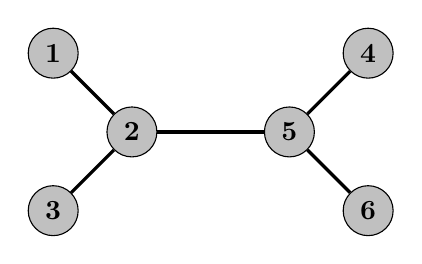
\begin{tikzpicture}
	\node[circle,draw=black,fill=gray] (1) at (-2,1) {\textbf{1}};
	\node[circle,draw=black,fill=gray] (2) at (-1,0) {\textbf{2}};
	\node[circle,draw=black,fill=gray] (3) at (-2,-1) {\textbf{3}};
	\node[circle,draw=black,fill=gray] (4) at (2,1) {\textbf{4}};
	\node[circle,draw=black,fill=gray] (5) at (1,0) {\textbf{5}};
	\node[circle,draw=black,fill=gray] (6) at (2,-1) {\textbf{6}};
	
	\foreach \x/\y in {1/2,2/3,2/5,4/5,5/6}
		\draw[black,=>latex',very thick] (\x) -- (\y);
\end{tikzpicture}%
}
\caption{A tree graph of order $6$.}
\label{fig:tree-graph}
\end{figure}

In 1984, Wiener strengthened the result in Theorem~\ref{thm:parter}~\cite{Wiener1984}.
This stronger result, stated in Theorem~\ref{thm:parter-wiener}, is now referred to as the Parter-Wiener theorem.
%%%%%%%%%%%%%%%%
%					Theorem 3.4	%
%%%%%%%%%%%%%%%%
\begin{theorem}\label{thm:parter-wiener}
Let $T$ be a tree and $A\in\mathcal{S}(T)$ with $\nullity{A}\geq 2$. 
Then, there is a vertex $i\in V(T)$ such that $\nullity{A(i)} = \nullity{A} + 1$, and the principal submatrices of $A$ corresponding to at least three branches of $T$ at $i$ are singular.
\end{theorem}

Note that $A(i)$ is the principal submatrix of $A$ obtained by deleting row and column $i$ from the matrix $A$. 
Moreover, the vertex $i$ for which $\nullity{(A-\lambda I)(i)} = \nullity{A-\lambda I}+1$ is known as a Parter-Wiener vertex for $A$ corresponding to the eigenvalue $\lambda$.
For example, the adjacency matrix of the tree graph in Figure~\ref{fig:tree-graph} has Parter-Wiener vertices $2$ and $5$ corresponding to the eigenvalue $0$.
Over the subsequent years, the Parter-Wiener theorem has been further developed and produced many beautiful results, e.g., see Chapter 2 of~\cite{Johnson2018}.

Nylen appears to be the first to study the minimum rank of a graph, which appeared in his 1996 paper~\cite{Nylen1996}.
In that paper, Nylen made the following observations.
%%%%%%%%%%%%%%%%
%					Proposition 3.5	%
%%%%%%%%%%%%%%%%
\begin{proposition}\label{prop:nylen}
Let $G\in\mathbb{G}$ have order $n\geq 1$.
Then,
\begin{enumerate}[a.]
\item If $A\in\mathcal{S}(G)$ and $v\in V(G)$, then the principal submatrix $A(v)$ corresponds to the induced subgraph $G-v$.
\item If $G$ is disconnected with connected components $G_{1},~G_{2},~\ldots,~G_{k}$, then
\[
mr(G) = \sum_{i=1}^{k}mr(G_{i}).
\]
\item If $G$ has $k$ connected components, then
\[
mr(G) \leq n-k.
\]
\item For each vertex $v\in V(G)$, we have
\[
mr(G) - 2 \leq mr(G-v) \leq mr(G).
\]
\item For each edge $e\in E(G)$, we have
\[
mr(G) - 1 \leq mr(G-e) \leq mr(G) + 1.
\]
\end{enumerate}
\end{proposition}

In addition, Nylen proved the following more substantial result.
%%%%%%%%%%%%%%%%
%					Theorem 3.6	%
%%%%%%%%%%%%%%%%
\begin{theorem}\label{thm:nylen}
Let $G\in\mathbb{G}$ and $A\in\mathcal{S}(G)$ with $\rank{A} = mr(G)$.
Then, for any vertex $i\in V(G)$, either $\rank{A(i)} = mr(G)-2$ or $\rank{A(i)} = mr(G)$.
\end{theorem}

The rest of Nylen's paper focuses on trees; in particular, he proved the following result, which provides an algorithm for computing the minimum rank of a tree.
Note that a \emph{high-degree} vertex of a graph is a vertex with degree at least $3$; a \emph{Nylen path} in a forest $F$ is a path with at most one high-degree vertex, and whose initial and terminal vertices each have degree $1$.
%%%%%%%%%%%%%%%%
%					Theorem 3.7	%
%%%%%%%%%%%%%%%%
\begin{theorem}\label{thm:nylen2}
Let $P$ be a Nylen path of the forest $F$.
Then,
\begin{enumerate}[a.]
\item If $P$ has a high-degree vertex $v$, then $mr(F) = mr(F-i)+2$.
\item If $P$ does not have a high-degree vertex, then $mr(F) = \abs{V(P)}-1 + mr(F-V(P))$.
\end{enumerate}
\end{theorem}
%%%%%%%%%%%%%%%%%%%%%%%%%%%%%%%%%%%%%%%%%%%%%%%%%%%%%%
%								Colin de Verdi{\'e}re Type Parameters
%%%%%%%%%%%%%%%%%%%%%%%%%%%%%%%%%%%%%%%%%%%%%%%%%%%%%%
\section{Colin de Verdi{\'e}re Type Parameters}

%%%%%%%%%%%%%%%%%%%%%%%%%%%%%%%%%%%%%%%%%%%%%%%%%%%%%%
%								Computational Approaches to Zero Forcing Number
%%%%%%%%%%%%%%%%%%%%%%%%%%%%%%%%%%%%%%%%%%%%%%%%%%%%%%
\section{Computational Approaches to Zero Forcing Number}

%%%%%%%%%%%%%%%%%%%%%%%%%%%%%%%%%%%%%%%%%%%%%%%%%%%%%%
%								Integer Program
%%%%%%%%%%%%%%%%%%%%%%%%%%%%%%%%%%%%%%%%%%%%%%%%%%%%%%
\subsection{Integer Program}
In this section, we review the integer program model introduced by Brimkov et al.~\cite{Brimkov2019} to compute the zero forcing number of a graph $G\in\mathbb{G}$.
This integer program is shown in~\eqref{eq:zfip-obj}--\eqref{eq:zfip-const4}, and we reference this program by $\zip{G}$.
Note that every edge in $E(G)$ is replaced by two directed edges with opposite direction.
A binary variable $s_{v}$ indicates whether vertex $v$ is in the zero forcing set; an integer variable $x_{v}$ ranging in $\{0,\ldots,T\}$ indicates at which timestep vertex $v$ is forced, where $T$ is the maximum difference between the forcing times of two vertices; finally, a binary variable $y_{e}$ for each directed edge $e = (u,v)$ indicates whether $u$ forces $v$.
The notation $\delta^{-}(v)$ refers to the set of edges pointing towards the node $v$, $N(u)$ denotes the open neighborhood of $u$, i.e., all vertices $v\in V(G)$ that are adjacent to $u$, and $N[u]$ denotes the closed neighborhood of $u$, i.e., $N[u] = N(u)\cup\{u\}$.
%%%%%%%%%%%%%%%%
%	Zero Forcing IP Model	%
%%%%%%%%%%%%%%%%
\begin{mini!}
	{}{\sum_{v\in V}s_{v}}{}{}\label{eq:zfip-obj}
	\addConstraint{s_{v}+\sum_{e\in\delta^{-}(v)}y_{e}}{=1,~\quad\forall v\in V}\label{eq:zfip-const1}
	\addConstraint{x_{u}-x_{v}+(T+1)y_{e}}{\leq T,~\quad\forall e=(u,v)\in E}\label{eq:zfip-const2}
	\addConstraint{x_{w}-x_{v}+(T+1)y_{e}}{\leq T,~\quad\forall e=(u,v)\in E,~\forall w\in N(u)\setminus\{v\}}\label{eq:zfip-const3}
	\addConstraint{s\in\{0,1\}^{n},~x\in\{0,\ldots,T\}^{n},~y\in\{0,1\}^{m}}{}\label{eq:zfip-const4}
\end{mini!}
The triple $(s,x,y)$, where $s\in\{0,1\}^{n},~x\in\{0,\ldots,T\}^{n},~y\in\{0,1\}^{m}$, is a \emph{feasible solution} of $\zip{G}$ provided that $s,x,y$ satisfy~\eqref{eq:zfip-const1}--\eqref{eq:zfip-const4}.
If, in addition, $s$ is minimal with respect to the objective function~\ref{eq:zfip-obj}, then we say that $(s,x,y)$ is an \emph{optimal solution} of $\zip{G}$.
The corresponding minimal value of the objective function~\ref{eq:zfip-obj} is the optimal value of $\zip{G}$.

%%%%%%%%%%%%%%%%
%					Theorem 5.1		%
%%%%%%%%%%%%%%%%
\begin{theorem}\label{thm:zfip}
Let $G\in\mathbb{G}$.
The optimal value of $\zip{G}$ is equal to the zero-forcing number of $G$.
\end{theorem}
\begin{proof}
Let $B\subseteq V$ denote a zero-forcing set of $G$.
Also, fix some chronological list of forces that results in a total coloring of $G$, and let $\mathcal{F}$ be the associated set of forcing chains. 
Since $B$ is a zero forcing set, every vertex $v\in V(G)$ is either in $B$, i.e., $s_{v}=1$, or is forced by some other vertex $u\in V(G)$, i.e., $y_{e}=1$ where $e=(u,v)$.
Thus, constraint~\eqref{eq:zfip-const1} must hold.
Now, let $x_{v}$ be the time step in which $v\in V(G)$ is forced. 
Since a vertex cannot force until all but one of its neighbors are forced, it follows that for every edge $e = (u,v)$ for which $y_{e}=1$, $u$ must be forced before $v$, i.e., $x_{u}<x_{v}$. 
Similarly, $x_{w}<x_{v}$ for all neighbors $w$ of $u$. 
Thus, constraints~\eqref{eq:zfip-const2} and~\eqref{eq:zfip-const3} are satisfied.
If $y_{e}=0$, then constraints~\eqref{eq:zfip-const2} and~\eqref{eq:zfip-const3} hold since $T$ is the maximum difference between the forcing times of two vertices. 
Therefore, constraints~\eqref{eq:zfip-const1}--\eqref{eq:zfip-const4} are valid for any zero-forcing set $B$ and associated set of forcing chains $\mathcal{F}$.

Conversely, let $(s,x,y)$ be a feasible solution of $\zip{G}$.
Define $B\subseteq V(G)$ to be the set of vertices for which $s_{v}=1$. 
By constraint~\eqref{eq:zfip-const1}, each vertex $v\in V(G)$ is either in $B$ or is the head of exactly one edge $e = (u,v)$ such that $y_{e}=1$.
Consider any such edge; then, by constraints~\eqref{eq:zfip-const2} and~\eqref{eq:zfip-const3}, there must be an integer $x_{v}\in\{0,\ldots,T\}$ such that $x_{w}+1\leq x_{v}$ for all $w\in N[u]\setminus\{v\}$. 
Therefore, the edges $e=(u,v)$ for which $y_{e}=1$ define a chronological list of forces.
Since every vertex $v\in V(G)$ is either in $B$ or is the head of exactly one edge $e = (u,v)$ such that $y_{e}=1$, it follows that $B$ is a zero-forcing set. 
If, in addition, $s$ is minimal with respect to the objective function~\eqref{eq:zfip-obj}, i.e., $(s,x,y)$ is an optimal solution of $\zip{G}$, then $B$ is a minimal zero-forcing set and it follows that the objective value of $\zip{G}$ is the zero-forcing number of $G$.
\end{proof}

%%%%%%%%%%%%%%%%%%%%%%%%%%%%%%%%%%%%%%%%%%%%%%%%%%%%%%
%								Heuristics
%%%%%%%%%%%%%%%%%%%%%%%%%%%%%%%%%%%%%%%%%%%%%%%%%%%%%%
\subsection{Heuristics}
In this section, we review a heuristic method for the zero-forcing number of a graph from~\cite{Brimkov2021}.
This heuristic is based on adding vertices to a set in order to maximize its closure.
Let $G = (V,E)$ be a simple graph and let $\mathcal{S}\subseteq V$ be an initial set of blue vertices.
The closure of $\mathcal{S}$, denoted $cl(\mathcal{S})$, is the set of blue vertices obtained after applying the color change rule until no other white vertices can be forced blue. 
Note that $\mathcal{S}$ is a zero-forcing set of $G$ if $cl(\mathcal{S}) = V$. 

In Algorithm~\ref{alg:heuristic}, $\mathcal{S}\subseteq V$ denotes a set of blue vertices and let $\mathcal{C}$ denotes the closure of $\mathcal{S}$. 
Note  that $\mathcal{S}$ is initialized as the empty set and grows on each iteration of the while loop until its closure, $\mathcal{C}$, is equal to $V$. 
In particular, on each iteration of the while loop, a set $A^{*}$ is computed that maximizes the function $f$ over certain sets of white vertices. 

%%%%%%%%%%%%%%%%%%%%%%%%
%						Algorithm 2.1						%
%%%%%%%%%%%%%%%%%%%%%%%%
\begin{algorithm}
\caption{Heuristic method for the zero-forcing number.}
\label{alg:heuristic}
\begin{algorithmic}
\STATE{Given a graph $G=(V,E)$, this algorithm returns a zero-forcing of $G$.}
\STATE{$\mathcal{S}\gets\emptyset$}
\STATE{$\mathcal{C}\gets\emptyset$}
\WHILE{$\mathcal{C}\neq V$}
	\STATE{$\mathcal{C}^{*}\gets\emptyset$}
	\STATE{$\mathcal{A}^{*}\gets\emptyset$}
	\FOR{$v\in V\setminus{\mathcal{C}}$}
		\STATE{$\mathcal{S}\gets \mathcal{C}\cup A(v,\mathcal{C})$}
		\IF{$f(cl(\mathcal{S}),v,\mathcal{C}) > f(C^{*},v,C)$}
			\STATE{$A^{*}\gets A(v,\mathcal{C})$}
			\STATE{$C^{*}\gets cl(\mathcal{S})$}
		\ENDIF
	\ENDFOR
	\STATE{$\mathcal{C}\gets\mathcal{C}^{*}$}
	\STATE{$\mathcal{S}\gets\mathcal{S}\cup\mathcal{A}^{*}$}
	\FOR{$v\in\mathcal{S}$}
		\IF{$cl(\mathcal{S}\setminus{\{v\}} = V$}
			\STATE{$\mathcal{S}\gets\mathcal{S}\setminus{\{v\}}$}
		\ENDIF
	\ENDFOR
\ENDWHILE
\end{algorithmic}
\end{algorithm}
%%%%%%%%%%%%%%%%%%%%%%%%%%%%%%%%%%%%%%%%%%%%%%%%%%%%%%
%								Propagation Time and Throttling Number
%%%%%%%%%%%%%%%%%%%%%%%%%%%%%%%%%%%%%%%%%%%%%%%%%%%%%%
\section{Propagation Time and Throttling Number}
Given a color change rule and a graph $G$, the propagation time of $B\subseteq V(G)$, denoted $pt(G,B)$, is the smallest $t$ such that $B^{[t]}=V(G)$ or $\infty$ if $B$ is not a zero-forcing set.
The propagation time of $G$ is defined by
\[
pt(G) = \min\left\{pt(G,B)\colon\text{$B$ is a minimal zero-forcing set}\right\}.
\]
In Figure~\ref{fig:tree-graph-coloring}, we illustrate the standard propagation process and blue sets $B^{[i]}$ for a tree $T$ and initial set $B=B^{[0]}$ such that $pt(T) = pt(G,B)$.
%%%%%%%%%%%%%%%%
%					Figure 5			%
%%%%%%%%%%%%%%%%
\begin{figure}[ht]
\centering
\resizebox{0.75\textwidth}{!}{% Tree Graph Coloring
\begin{tabular}{ccc}
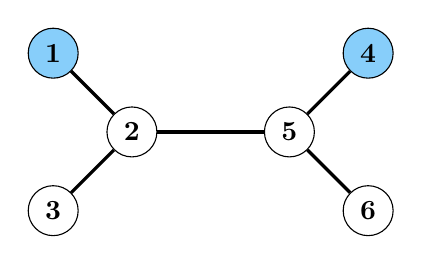
\begin{tikzpicture}
	\node[circle,draw=black,fill=sky_blue] (1) at (-2,1) {\textbf{1}};
	\node[circle,draw=black,fill=white] (2) at (-1,0) {\textbf{2}};
	\node[circle,draw=black,fill=white] (3) at (-2,-1) {\textbf{3}};
	\node[circle,draw=black,fill=sky_blue] (4) at (2,1) {\textbf{4}};
	\node[circle,draw=black,fill=white] (5) at (1,0) {\textbf{5}};
	\node[circle,draw=black,fill=white] (6) at (2,-1) {\textbf{6}};
	
	\foreach \x/\y in {1/2,2/3,2/5,4/5,5/6}
		\draw[black,=>latex',very thick] (\x) -- (\y);
\end{tikzpicture}
&
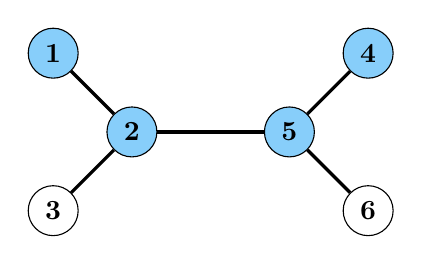
\begin{tikzpicture}
	\node[circle,draw=black,fill=sky_blue] (1) at (-2,1) {\textbf{1}};
	\node[circle,draw=black,fill=sky_blue] (2) at (-1,0) {\textbf{2}};
	\node[circle,draw=black,fill=white] (3) at (-2,-1) {\textbf{3}};
	\node[circle,draw=black,fill=sky_blue] (4) at (2,1) {\textbf{4}};
	\node[circle,draw=black,fill=sky_blue] (5) at (1,0) {\textbf{5}};
	\node[circle,draw=black,fill=white] (6) at (2,-1) {\textbf{6}};
	
	\foreach \x/\y in {1/2,2/3,2/5,4/5,5/6}
		\draw[black,=>latex',very thick] (\x) -- (\y);
\end{tikzpicture}
&
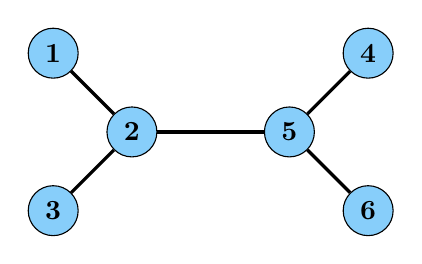
\begin{tikzpicture}
	\node[circle,draw=black,fill=sky_blue] (1) at (-2,1) {\textbf{1}};
	\node[circle,draw=black,fill=sky_blue] (2) at (-1,0) {\textbf{2}};
	\node[circle,draw=black,fill=sky_blue] (3) at (-2,-1) {\textbf{3}};
	\node[circle,draw=black,fill=sky_blue] (4) at (2,1) {\textbf{4}};
	\node[circle,draw=black,fill=sky_blue] (5) at (1,0) {\textbf{5}};
	\node[circle,draw=black,fill=sky_blue] (6) at (2,-1) {\textbf{6}};
	
	\foreach \x/\y in {1/2,2/3,2/5,4/5,5/6}
		\draw[black,=>latex',very thick] (\x) -- (\y);
\end{tikzpicture}
\\$B^{[0]} = \{1,4\}$ & $B^{[1]} = \{1,2,4,5\}$ & $B^{[2]} = \{1,2,3,4,5,6\}$ \\
\end{tabular}%
}
\caption{A zero forcing set for a tree graph of order $6$.}
\label{fig:tree-graph-coloring}
\end{figure}

Given a color change rule and a graph $G$, the throttling number of $B\subseteq V(G)$ is defined by
\[
th(G,B) = \abs{B} + pt(G,B).
\]
Furthermore, the throttling number of $G$ is defined by
\[
th(G) = \min_{B\subseteq V(G)} th(G,B).
\]
Note that throttling number is not necessarily attained for minimal zero-forcing sets. 
Indeed, consider the path graph of order $n$, denoted by $P_{n}$. 
Note that $Z\left(P_{n}\right)=1$, and any of the two leafs in $P_{n}$ will serve as a zero forcing set, e.g., see Figure~\ref{fig:path-graph-coloring}. 
Since every other node will be forced, one at a time, it follows that $pt\left(P_{n},B\right)=n-1$, for any minimal zero-forcing set. 
Therefore,
\[
th\left(P_{n},B\right) = n
\]
for any minimal zero-forcing set $B$. 
However, if we let the initial coloring $B$ be made up of both leafs in $P_{n}$, then $pt\left(P_{n},B\right)=\lceil (n-2)/2 \rceil$, and it follows that
\[
th\left(P_{n},B\right) = 2 + \lceil (n-2)/2 \rceil.
\]
Therefore, $th\left(P_{n}\right) < n$ for all $n>3$. 
%%%%%%%%%%%%%%%%%%%%%%%%%%%%%%%%%%%%%%%%%%%%%%%%%%%%%%
%                                 	   			Bibliography
%%%%%%%%%%%%%%%%%%%%%%%%%%%%%%%%%%%%%%%%%%%%%%%%%%%%%%
\label{Bibliography}
\bibliographystyle{siam}
\bibliography{Bibliography}

\end{document}